\documentclass{article}
\usepackage{graphicx} % Required for inserting images
\usepackage{float}
\usepackage[utf8]{inputenc}
\usepackage[T1]{fontenc}
\usepackage{pdfpages}

\title{Rapport í Linux Skipanir}
\author{Salomon Vágadal Joensen, 2022.210\\Jákup Paulason Olsen, 2020.006\\Helena Hentze, 2022.197}
\date{1. Marts 2024}

\begin{document}
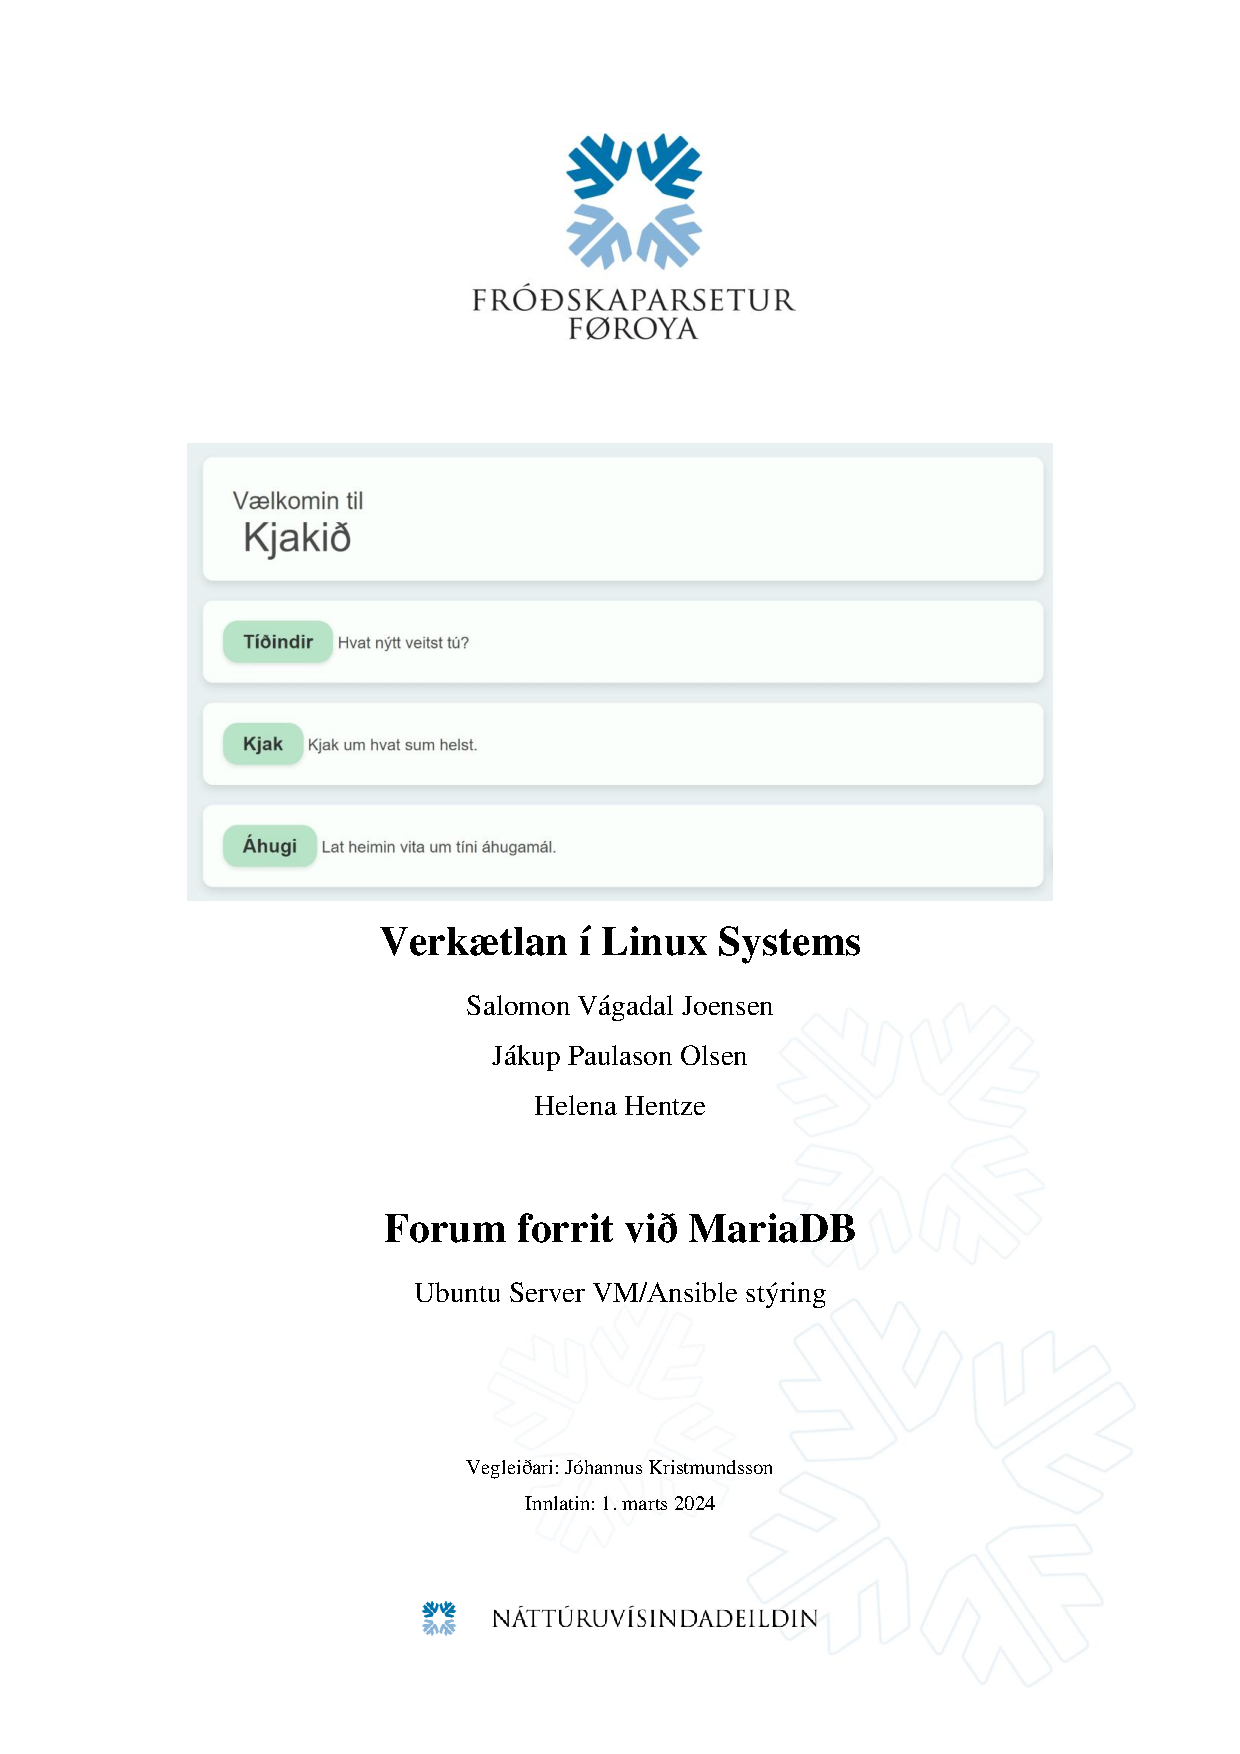
\includepdf[pages=-]{Rapport_frontpage_kjakid.pdf}
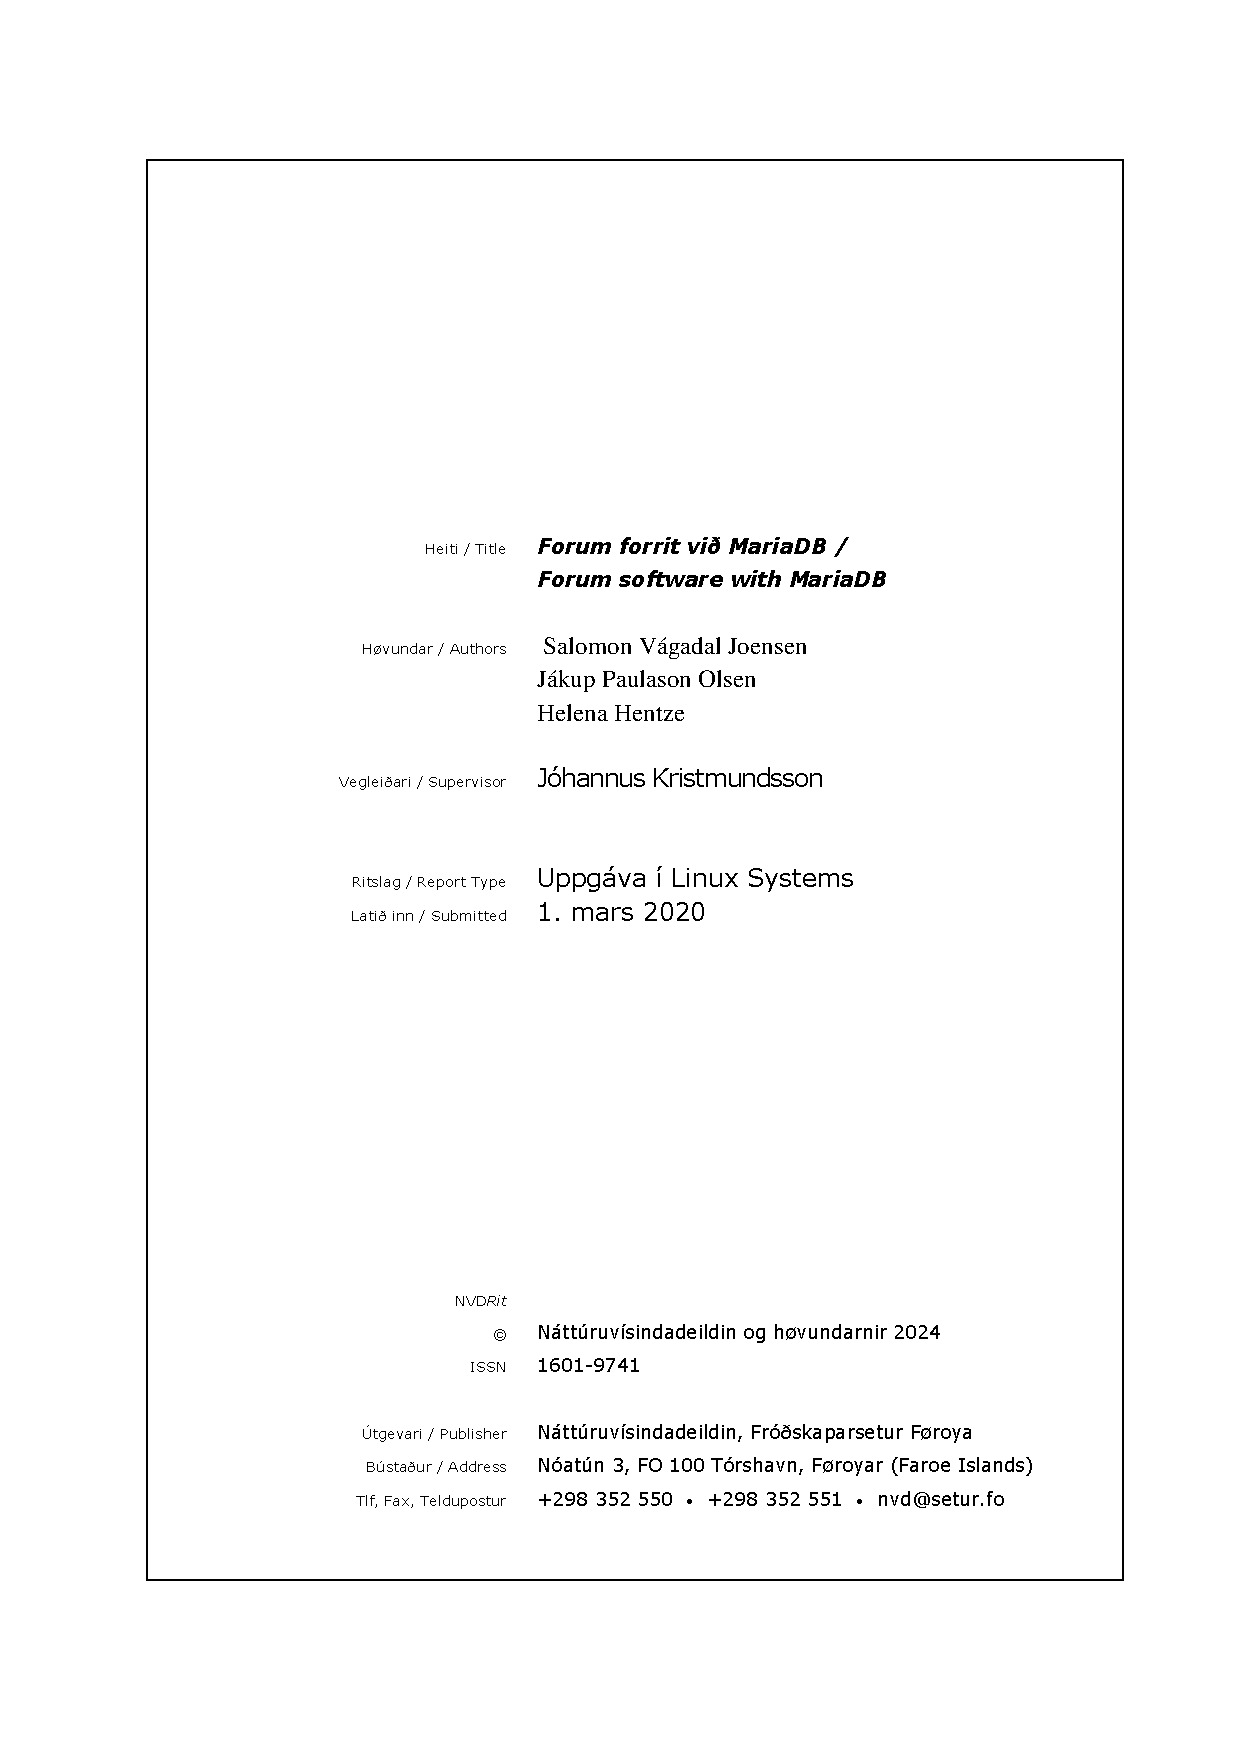
\includepdf[pages=-]{titlepage_kjakid.pdf}
%\maketitle

\section{Problemformulering}
\par Hvussu ger man eina kjak heimasíðu sum fólk kunnu vitja og stovna tráðir og leggja innlegg í? Og møguliga eisini hava møguleika at deila media har? 
\begin{itemize}
    \item Man má gera sær greitt at har má vera ein heimasíða, sum fólk vitja.
    \item Á hesari heimasíðuni skal brúkarin kunna síggja kjaksíður.
    \begin{itemize}
        \item Fara inn á eina kjak undirsíðu.
        \item Síggja tráðir og kunna stovna tráðir.
        \item Kunna fara inn á einkultar tráðir og svara í einum tráði og viðmerkja navn, tekstsvar og um tey vilja leggja mynd avtrat. 
    \end{itemize}
\end{itemize} 

\section{Tólmenni}
\par Ein Ubuntu Server við einari lokalari heimasíðu og brúkt ein MariaDB dátagrunn
at goyma tráðirnir og postar í.
PhpMyAdmin verður brúkt til at síggja dátagrunnin og tað er installera á sjálva servaran,
men er ikki partur av Ansible playbook, tí tað er ikki neyðugt fyri at fáa kjak heimasíðuna
at virka.

\section{Mál / Framgangsháttur}
\par Vit byrja við einari stutta analysu hvussu hetta skal fremjast.
\begin{itemize}
    \item Arkitektur bygnaða av probleminum og hvussu tað fer at síggja út.
    \item Gera ein databasa í MariaDB har man kann stovna ein \textit{thread} í 3 ymiskum kjakforum har fólk kunna svara uppá.
    \item Við einum fullfíggjaðum MariaDB datagrunn byggja eina heimasíðu sum virkar sum eitt \textit{interface} millum heimasíðuna og datagrunnin.
    \item \textit{Business logic} millumlið verður brúkt PHP til samskifting millum
            \newline heimasíðuna og MariaDB.
    \item Millumliðið fer at avgera hvussu úrslit frá datagrunninum verður víst.
    
\end{itemize}

\section{Design}
\begin{figure}[H]
    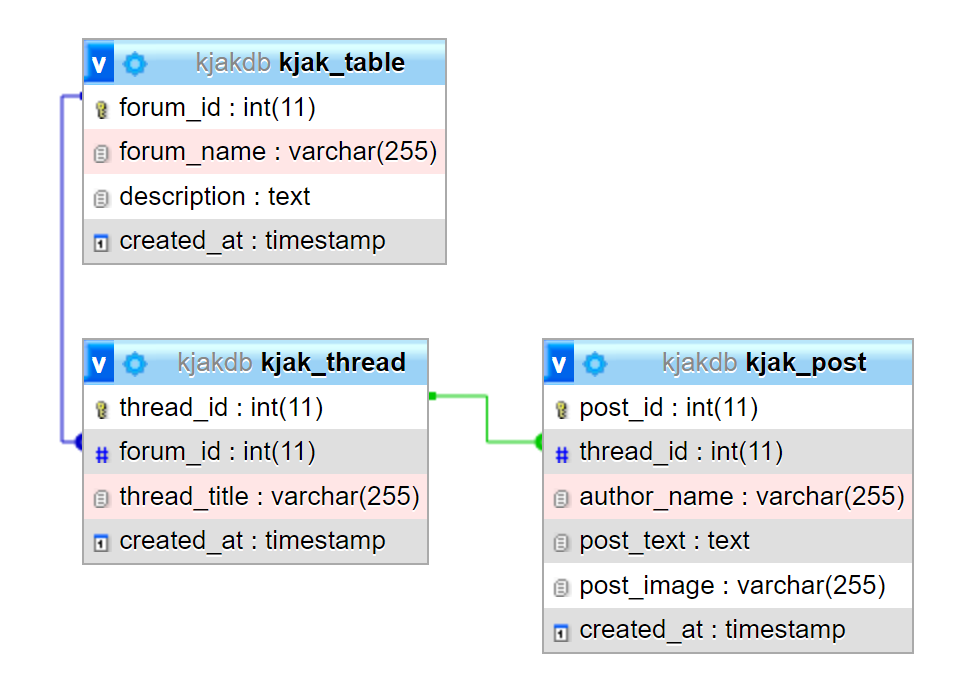
\includegraphics[width=\linewidth]{kjakdb_table_relations.png}
    \caption{Databasa relatiónirnar fyri \textit{kjakdb}}
    \label{fig:kjakdb_table_relations}
\end{figure}

\par Databasa relatiónirnar vísa hvussu
tær 3 tabelirnar eru relatarar. \textbf{kjak\_table} er høvuðs tabellin og hevur
\textit{Primary Key} \underline{forum\_id} til \textit{Foreign Key} til \textbf{kjak\_thread},
og \textbf{kjak\_thread} hevur \textit{Primary Key} \underline{thread\_id} til \textit{Foreign Key}
til \textbf{kjak\_post}.
 
\par Heimasíðan er bert 4 síður við embeddaða PHP kodu til at vísa dáta frá \textit{kjakdb}
dátagrunnins 3 tabellir. Annars er ein CSS fíl \textit{style.css} fyri uppseting
og ein \textit{conn.php} við
íbinding upplýsingarnar til dátagrunnin. Tær 4 síðurnar eru:
\begin{itemize}
    \item \textit{index.php} Heimasíðan sum vísur forumini.
    \item \textit{view\_forum.php} Undirsíðan fyri at vísa tráðir fyri eitt forum.
    \item \textit{view\_thread.php} Undirsíðan fyri at vísa ein á tráð og allar svør í tí
            tráðinum.
    \item \textit{create\_thread.php} Fyri at stovna ein nýggjan tráð.
\end{itemize}

\section{Appendix}

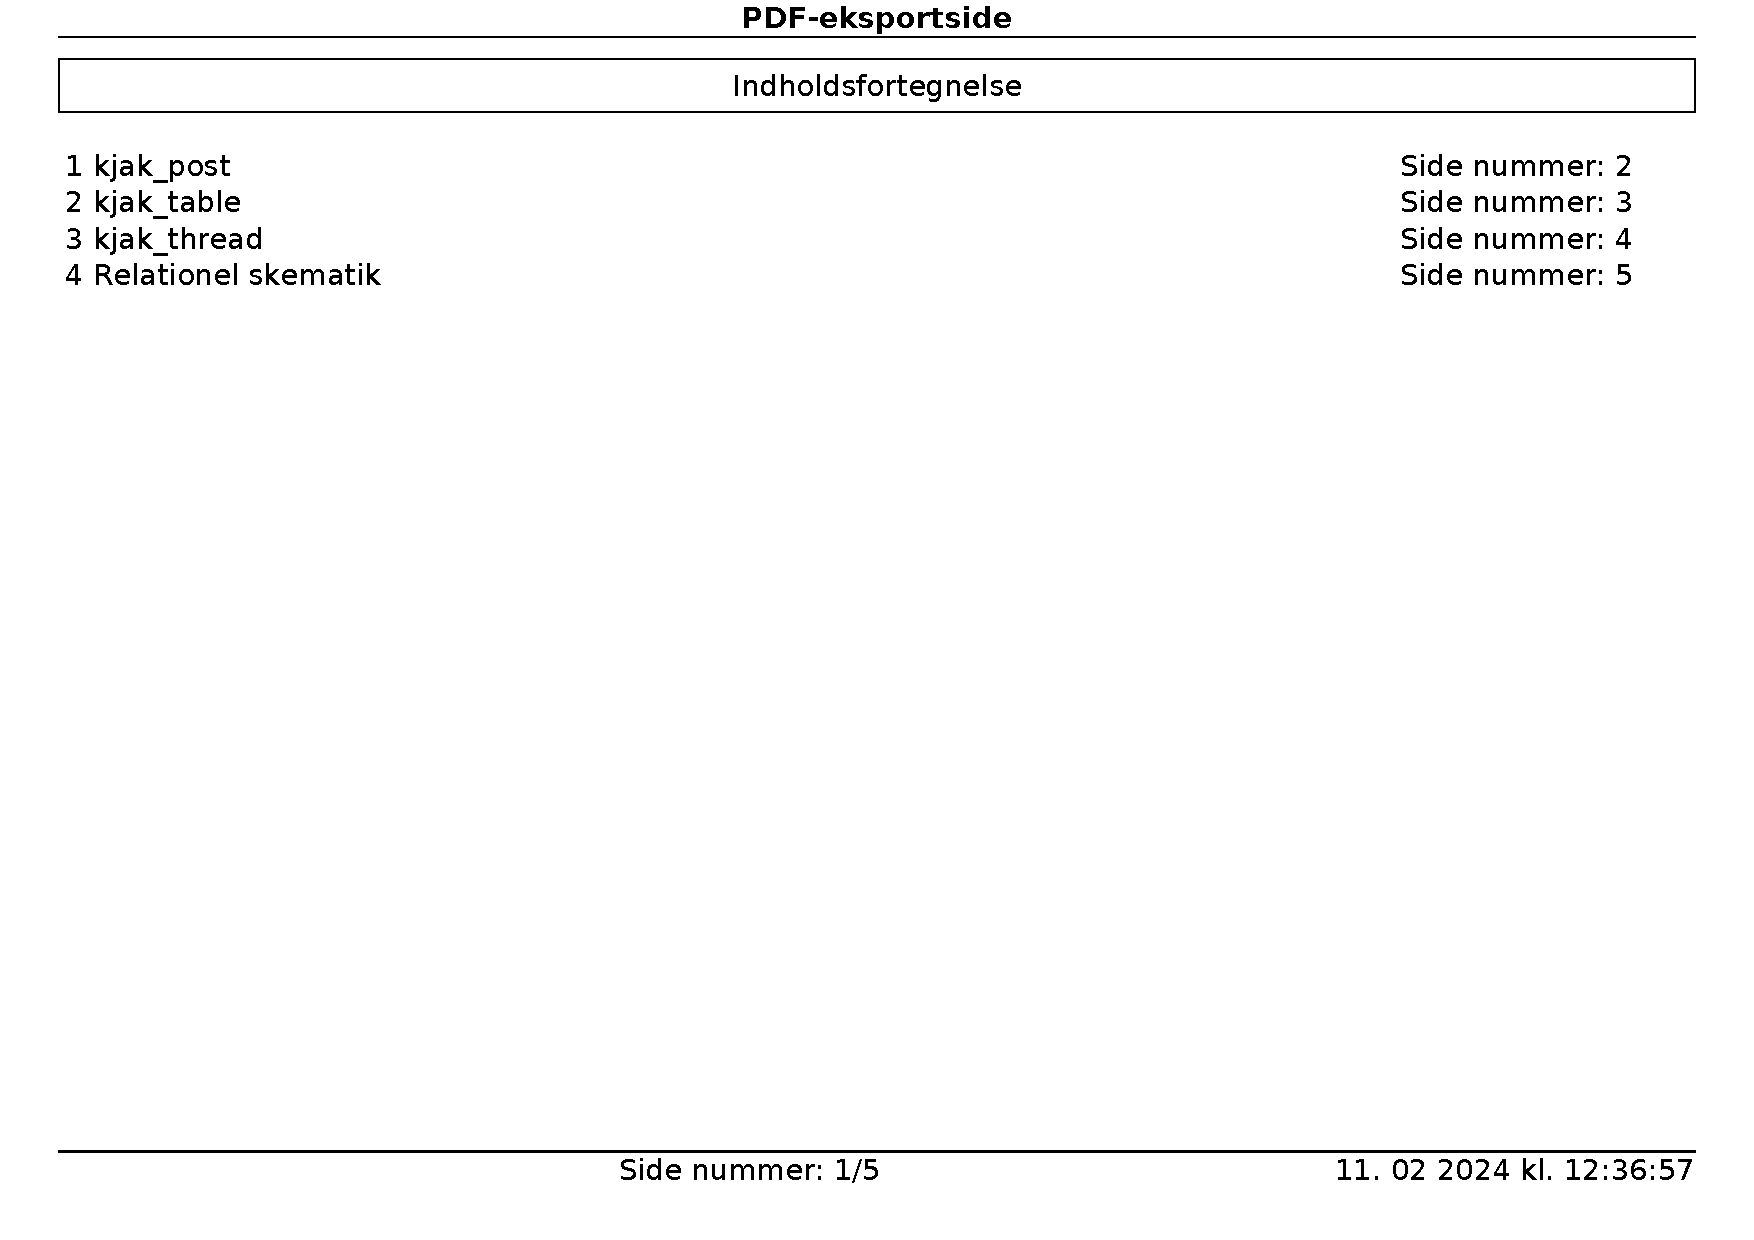
\includepdf[pages=-]{kjakdb_schema.pdf}

\end{document}
